%%
%% This is file `mcmthesis-demo.tex',
%% generated with the docstrip utility.
%%
%% The original source files were:
%%
%% mcmthesis.dtx  (with options: `demo')
%%
%% -----------------------------------
%%
%% This is a generated file.
%%
%% Copyright (C)
%%     2010 -- 2015 by Zhaoli
%%     2014 -- 2016 by Liam 
%%     2017 -- 2019 by Xuehan
%%
%% This work may be distributed and/or modified under the
%% conditions of the LaTeX Project Public License, either version 1.3
%% of this license or (at your option) any later version.
%%
%% This work has the LPPL maintenance status `maintained'.
%%
%% The Current Maintainer of this work is Xuehan.
%%
\documentclass{mcmthesis}
\bibliographystyle{IEEEtran}
\mcmsetup{CTeX = false,   % 使用 CTeX 套装时,设置为 true
        tcn = 2002134, problem = D,
        sheet = true, titleinsheet = true, keywordsinsheet = true,
        titlepage = true}
\usepackage{palatino}
\usepackage{mwe}
\usepackage{graphicx}
\usepackage{subcaption}
\usepackage{float}
\usepackage{multirow}
\usepackage{indentfirst}
\usepackage{gensymb}
\usepackage[ruled,lined,commentsnumbered]{algorithm2e}
\usepackage{geometry}
\usepackage{amsmath}
\usepackage{array}
\usepackage{pythonhighlight}

\begin{document}
\linespread{0.6} %%行间距
\setlength{\parskip}{0.5\baselineskip} %%段间距
\title{ti}

\date{\today}
	\begin{abstract}

	
		\begin{keywords}
		
		\end{keywords}
	\end{abstract}

\maketitle

\tableofcontents

\newpage

\section{Introduction}
\subsection{Problem Background}
	Football is one of the most well-known sports activities in the world.  The standard system of an 11-man football game is one goalkeeper and 10 players from each of the two teams. There are a total of 22 players who fight, defend and attack on the rectangular grass court.  The game scores by shooting the ball into the opponent's goal. When the game is over, the team with the most points wins.

	\begin{figure}[h]
		\centering
		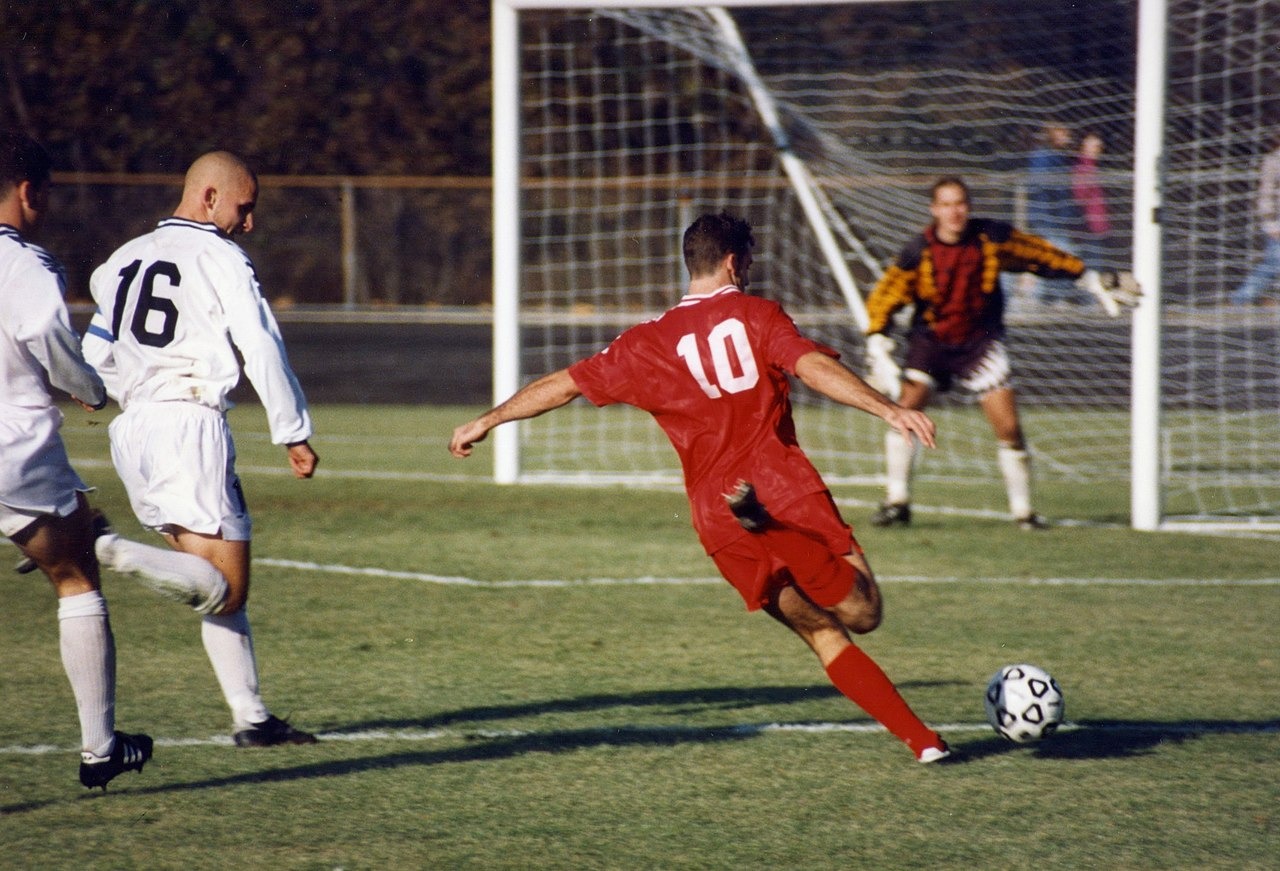
\includegraphics[width=0.75\textwidth]{figures/football.jpg}
		\caption{A Football Game~\cite{Wiki_Football}}
		\label{fig:football}
	\end{figure}

	As we all know, football is a sport that requires intense teamwork.  For it can show the importance of teamwork spirit more than superb personal ability.  Passing, as an offensive means that requires the cooperation of various players to play the biggest role, is just an important manifestation of the team spirit of football.  Therefore, to study the important role of teamwork in football, we will start by studying the passing network in football.

	Our goal is to build a network model to simulate the Huskies' passing network and study it.  Meanwhile, it is necessary to extract some representative parameters from the constructed network model.  Through the study of such parameters, we can accurately understand the team collaboration ability and structural characteristics of this team.
\subsection{Our Work}
	In this paper, we successfully built the Huskies' passing network model.  On the basis of this network model, we obtained some important parameters. In this way, we analyzed the team collaboration ability of the Huskies players, and offered some suggestion for its future structural strategy.

	In Section 2, we state some basic assumptions.  Section 3 contains the nomenclature used in the statement of our model.  Section 4 provides sufficient details about our network model.  Section 5 carries on the simulation experiment and analysis to our proposed model.  Section 6 provides some advice on its structural strategies for the Huskies.  Finally, we further analyze the sensitivity, advantages and disadvantages of our model in Section 7, and we obtain some conclusions on how to improve the teamwork spirit of general teams in Section 8.
\section{Assumptions}
	Our model is based on these following basic assumptions:
	\begin{enumerate}
		\item The average position of a player over a period of time is equivalent to the average of the position of the player in all events that occurred during that period.
		\item We consider a dyadic configuration tight if this kind of dyadic configuration appears far more often than others.  The same is true for triadic configurations.
	\end{enumerate}
\section{Nomenclature}
	Symbols that our model mainly uses are listed in Table \ref{tab:Nomen}.  Other symbols that are used only once will be described in the following chapters.
	\begin{table}
    	\centering
    	\caption{Nomenclature}
		\label{tab:Nomen}
		\begin{tabular}{c c}
			\hline	
				Symbol & Definition\\
			\hline
				$\textbf{A}$ & Football passing matrix\\
				$\textbf{B}$ & Adjacency matrix\\
				$G$ & Undirected graph representing the football passing network\\
				$p_{i}$ & The \emph{i}th player in Huskies\\
				$w_{ij}$ & Number of passes from player $i$ to player $j$\\
				$\langle$$X$$\rangle$ & The x-coordinate of the network centroid\\
				$\langle$$Y$$\rangle$ & The y-coordinate of the network centroid\\
				$D$ & The dispersion of the position of the players around the network centroid\\
				$r$ & The advance speed\\
				$\textbf{L}$ & The Laplacian matrix\\
				$\lambda_{1}$ & the largest eigenvalue of the football passing matrix\\
				$\lambda_{2}$ & The second smallest eigenvalue of the Laplacian matrix\\
				$C$ & The clustering coefficient\\
				$d$ & The average shortest path\\
			\hline
   	 	\end{tabular}
	\end{table}

\section{The Basic Model}
	In this section we will discuss our network model in detail.  First of all, we will begin with the establishment of our network model.  Then we will use our model to identify some patterns of the network.  Finally, we will also investigate the indicators of teamwork. 
\subsection{Build of the Network}
	First of all, we define Huskies' football passing matrix $\textbf{A}$.  When the number of players who have played is $n$, $\textbf{A}$ is a square matrix of $n \times n$, which is defined as:
	\begin{equation}\label{eq:Mat_A}
		a_{ij} =
		\begin{cases}
			w_{ij}& \text{$i \neq j$}\\
			0& \text{$i = j$}
		\end{cases}
	\end{equation}
	In this way, we obtain an asymmetric square matrix of order $n$.  Next, on this basis, we try to build an undirected graph model to describe the team's passing network.  But as we have mentioned before, the adjacency matrix of an undirected graph is a symmetric matrix, while the football passing matrix $\textbf{A}$ we constructed is asymmetric.  Therefore, we need to construct a symmetric adjacency matrix $\textbf{B}$ using this asymmetric passing matrix $\textbf{A}$.  To achieve this, we define $\textbf{B}$ as the sum of $\textbf{A}$ and the transposed matrix of $\textbf{A}$, that is to say, for each element $b_{ij}$ in B, the following formula is satisfied:
	\begin{equation}
		\label{eq:Mat_B}
		b_{ij} = a_{ij} + a_{ji}
	\end{equation}
	Now we can easily find that $\textbf{B}$ is equal to its transpose matrix.  Hence $\textbf{B}$ is a symmetric matrix.

	After getting $\textbf{B}$, we can continue to study the undirected graph $G$.  From the previous definition of the adjacency matrix, it can be seen that the nodes in this undirected graph represent the Huskies players, and the edges represent interactions between players.  For quantitative research, we define the weight of node $i$ in the undirected graph $G$ as the sum of the number of passes and catches by player $i$, and the weight of edge $E (i, j)$ is defined as the sum of the number of passes from player $i$ to player $j$ and the number of passes from player $j$ to player $i$.
	
	In order to have an intuitive understanding of the football passing network, we can draw this undirected graph on a schematic diagram of a football field.  Among them, circles represent nodes, and straight lines connecting circles represent edges.  For a node, the larger its size and the darker its color, the greater the weight of the node.  For an edge, the thicker its thickness and the darker its color, the greater the weight of the edge.  In addition, in order to gain a clear understanding of the formation and other factors of this team, we plot the nodes on the represented player's the average position in the studied period.  In this way, we obtain a schematic diagram which can intuitively reflect the football passing network.  Figure \ref{fig:playground} is an example by us.
	
	\begin{figure}[h]
		\centering
		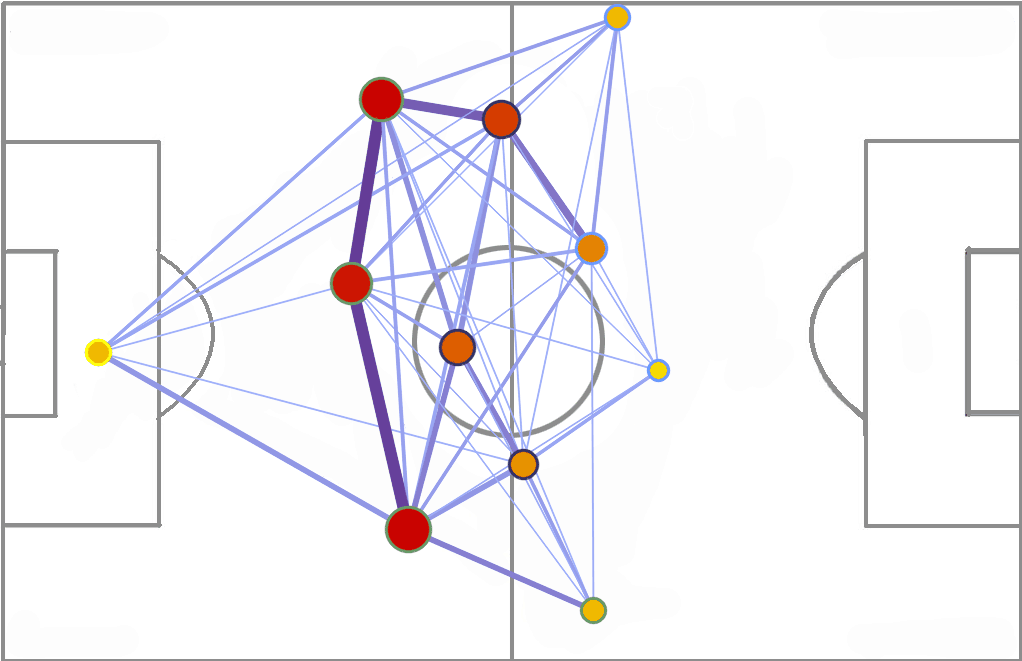
\includegraphics[width=0.7\textwidth]{figures/playground.png}
		\caption{An Example of the Football Passing Network}
		\label{fig:playground}
	\end{figure}
\subsection{Identify Network Patterns}
	After establishing the football passing network, we will use this model to identify some special patterns of Huskies' network.  In the following chapters, we will investigate Huskies' continuous football passing chain, network centroid and advance speed to identify its patterns on multiple scales. 
\subsubsection{Continuous Football Passing Chain}
	Just as we have stated in assumption 2, when players in a dyadic or triadic configuration continuously pass each other far more frequently than they do with other players in the team, we consider this configuration tight.  Therefore, when investigating the tightness of such configurations, we need to study the behavior of continuous passing between players.  For this reason, we construct a continuous football passing chain as a tool to study this behavior according to the football passing network.

	In football games, passing is a very continuous activity.  It can be said that before occasion like shooting, out of bounds or the football is intercepted by the opposing player occurs, the passing can build a transitive binary relationship between our players.  Therefore, we can use this characteristic to construct a continuous football passing chain, which is continuous and transitive.  The general construction method is: According to the data in passingevents, we record the process of continuous passing of football between Huskies players with a linked chain.  This chain will continue until disruptive occasions such as shooting, out of bounds or the football is intercepted by the opponent occur.  In this way, we get a chain that records the continuous passing of the Huskies players.

	From the continuous football passing chains, we can easily identify those tight dyadic and triadic configurations.  For example, if we want to identify a dyadic configuration, we can study these chains based on the characteristics that players in this dyadic configuration pass each other more frequently.  We can just number these two players we are studying as 0 and 1. In this way, there will be a large number of fragments like"0 - 1 - 0 - 1" or "0 - 1 - 0 - 1 - 0" in the continuous football passing chain.  If we want to identify those triadic configurations that are tight, we can just look for those fragments such as "0 - 1 - 2 - 1" or "0 - 1 - 2 - 0" from the continuous football pass chain.  Obviously, we can make similar judgments about multiple configurations.  Therefore, it will be convenient for us to find out which kind of configuration appears most.
\subsubsection{Network Centroid And Advance Speed}
	Studying the network centroid and advancing ratio of Huskies' football passing network will display the spatial features of the network better~\cite{First}.  In this section, we will study the coordinates of the network centroid of the football passing network constructed previously, the dispersion of the position of Huskies players around the network centroid, and the advance speed.

	We first study the coordinates of football passing network centroid.  According to the description of coordinates in readme, the x-coordinate on the field is oriented from the perspective of the team that is attacking, where 0 indicates the attacking team's own goal, and 100 indicates the oppositing team's goal.  While for y-coordinate, 0 indicates the attacking team's left-hand side, and 100 indicates its right-hand side.  We define the coordinates of a pass $(x_{i}, y_{i})$ as the average of the origin and destination positions.  Furthermore, we define the coordinates of the network centroid over a period of time as the average coordinates of all passes during that period.  It can be expressed as the following formula: 
	$$\langle X \rangle=\sum_{i=1}^n\frac{1}{n} x_{i}$$
	$$\langle Y \rangle=\sum_{i=1}^n\frac{1}{n} y_{i}$$
	The change of the network centroid coordinates over time can clearly reflect the overall movement tendency of the entire team during this time.  Besides,regardless of the length of the research period, it can always convey some information about the spatial features of the network.

	Then we continue to study the dispersion of the position of Huskies players around the network centroid.  Similarly, we define the dispersion of the position of Huskies players around the network centroid over a period of time $D$ as the variance between the average position of each player and the position of the network centroid during this period.  It can show how dispersed the team is on the court during this time.  Hence it can also reflect the degree of team control over the playing field during this time.  The greater the degree of dispersion, the stronger the team's ability to control the field.

	Finally, we define the team's advance speed over a period of time $r$ as the ratio of the sum of the absolute values ​​of the lateral displacement and the sum of the absolute values ​​of the longitudinal displacement of all its passes during that period. Its formula is:
	$$r=\frac{|\Sigma \Delta x|}{|\Sigma \Delta y|}$$
	The advance speed indicates the team's passing direction.  Besides, it can also reflect the team's movement tendency and offensiveness during this period.
\subsection{Identify Teamwork Indicators}
	In this part, we comprehensively use AHP analysis method for modeling, and use judgment matrix to choose the weight of each factor. Besides, all scores are normalized before weighting.

	We comprehensively analyze the composition of events on the court and abstract based on existing data, and propose the following model.  The model that captures structural, configurational, and dynamical aspects of teamwork mainly includes the following five aspects:
	\begin{itemize}
		\item Offensive score;
		\item Defensive score;
		\item Coordination score;
		\item Robustness score;
		\item Flexibility score.
	\end{itemize}
\subsubsection{Offensive Score}
	In theory, tactics do not have the so-called advantages and disadvantages. The quality of tactics should depend on whether they can work wonders.  Based on this, the evaluation of an offensive tactic should be based on the performance of the attacker, the performance of the defender, and some special situations.
	\begin{enumerate}
	\item The Performance of the Attacker
	
	\qquad The offense on the football field is nothing more than passing and shooting. Apart from cases that the player can shoot alone because of excellent personal strength, good offense should be the result of successful teamwork.  Therefore, the number of passes should be the main consideration. Pass is divided into simple pass, smart pass, head pass, high pass and hand pass. And the main ones that appear in the offense are simple pass and smart pass. Head pass and high pass will only appear in specific situations, so they are not considered here.

	\qquad At the same time, the ball possession rate in the opponent's penalty area is also an important indicator of the aggressiveness of the offense. As the defender's last area, the penalty area is unquestionably strong.  Defensively, every striker will be pressed by at least one person.  And there will even be double-jacketing and multiple-jacketing situations.Therefore, the statistics of the ball control rate here is of great significance. It can comprehensively reflect the quality of tactics.Good tactics should be those the team can still control the ball in the face of high-intensity defense.

	\qquad And for the opponent will defend for each attack, the perfect attack should be that pass more to minimize the confrontation, so the number of confrontations in each attack should also be considered.  Note that each confrontation in the event table occurs in pairs: ground attacking duel and ground defending duel.  Therefore, this pair is directly referred to as ground duel in our analysis.  But in the event statistics, as long as the offensive and defensive opponents face each other, the situation is counted as ground duel.  Hence the events after the ground duel should be counted. The general choice is to quickly pass the ball to others or choose to pass the ball by himselt with extraodinary skills, so these two indicators should be considered together.

	\qquad Then good tactics also have the option of making fouls. Making fouls in the penalty area can earn a free kick. At this time, the foul is really worth a thousand dollars, so we will also count the number of fouls in each attack.
	
	\qquad Based on this, the quantitative indicators are as follows:
	
	\begin{itemize}
		\item $\eta$ is the football possession time ratio;
		\item $p_{1}$ is the number of simple passes;
		\item $p_{2}$ is the number of smart passes;
		\item $n_{1}$ is the number of passes after ground duel;
		\item $n_{2}$ is the number of ground duels after ground duel;
		\item $n_{3}$ is the number of free kicks after making the opponent foul.
	\end{itemize}

	\qquad The corresponding judgment matrix is:
	\begin{equation}\label{mat:1}
		AP=
 	\begin{matrix}
   		 & \eta & p_{1} & p_{2} & n_{1} & n_{2} & n_{3} \\
   		\eta & 1 & 3 & 1 & 1 & 1 & \frac{1}{2} \\
		p_{1} & \frac{1}{3} & 1 & \frac{1}{3} & \frac{1}{3} &\frac{1}{3} &\frac{1}{7}\\
		p_{2} & 1 & 3 & 1 & 1 & 1 & \frac{1}{2} \\ 
		n_{1} & 1 & 3 & 1 & 1 & 1 & \frac{1}{2} \\ 
		n_{2} & 1 & 3 & 1 & 1 & 1 & \frac{1}{3} \\
		n_{3} & 2 & 7 & 2 & 2 & 3 & 1 
		
  	\end{matrix} 
	\end{equation}
	
	\item The Performance of the Defender
	
	\qquad The quality of an offense can also be judged from the other side, that is, the performance of the defensive end. The execution of an offensive tactic in place should theoretically fly the ball towards the goal and no opponent player blocks it.  At this time, the opponent team can only rely on the goalkeeper's response to try a save attempt.  Therefore, the defensive save attempt can also judge the quality of an offensive tactic.

	\begin{itemize}
		\item $d$ is the number of the opponent's save attempts.
	\end{itemize}

	\item Special Situations
	
	\qquad In some special cases, the tactics are just the front pavement. At that time, whether the goal can be achieved depends on the player ’s personal play and a certain degree of luck. In that case, it is usually a long corner kick, cross to the penalty area and rely on the player's aerial confrontation to pass the header, or run to the ball in advance to grab the ball and successfully shoot. In these cases, the tactics generally only prepare the first half, so it should be considered.

	\begin{itemize}
		\item $f$ is the number of shots right after crossing to the penalty area or right after corner.
	\end{itemize}

	\end{enumerate}
	
	The offensive tactics are scored by analyzing \textbf{the overall performance of the attacker, the performance of the defender, and the special situation}.The corresponding judgment matrix is:

	\begin{equation}\label{mat:2}
		OS=
	  \begin{matrix}
		& AP & d &f\\
   		AP & 1 & 1 & 2 \\
   		d & 1 & 1 & 2 \\
   		f & \frac{1}{2} & \frac{1}{2} & 1
  	\end{matrix}
	\end{equation}
	
\subsubsection{Defensive Score}
	\qquad For the event table cannot reflect the occupancy of each defensive player, there is no way to know which defensive strategy is actually used. Therefore we can only start from the event-driven and consider the location of each event to establish our model.
	\begin{enumerate}
	\item ODC
	
	\qquad ODC refers to the number of opponent's successful passes within 20 yards of Huskies' bottom line. This area is the core defense area and the last defense area for each team.  By judging the number of successful passes by the opponent within 20 yards of the bottom line, it can clearly reflect the level of the team's defensive level from the side, and it can also reflect the level of the team's defensive tactics. Good defensive tactics will make it impossible for the enemy players to find a point to cope with, which means that the number of successful passes will be reduced.

	\qquad Therefore, the smaller the ODC value, the better the defensive effect of this game. Limiting the opponent's offense can indicate that the defensive quality is great, and the frequency of threats to the defensive area of ​​this team's own side is low.

	\begin{itemize}
		\item $ODC$ is the number of successful passes within 20 yards of this team's own baseline.
	\end{itemize}

	\item PPDA
	
	\qquad In PPDA, defensive actions are defined in the following four areas: steals, interceptions, confrontations, and fouls.  In this indicator, we only consider the pressure exerted by the player when defending against the opponent, and not care about other issues.

	\qquad The smaller the value of PPDA, it means that the team's defensive strength is higher, and this also shows from a side that in this particular area, the chances of the offensive team wanting to use the pass to tear the defensive team's defense line are relatively small.

	\qquad Of course, it is impossible for any team that adopts pressure defense to adopt such a strategy throughout the entire game. Most of the time, pressure defense has a trigger point, such as a player entering a specific area (this is also called trigger switch).  However, if all these factors are taken into account, the project volume will be quite huge, and some artificial subjective factors will be mixed into it.  Therefore, in the "defense strength" indicator, we will only provide an objective data, which is measured by all the defensive actions and the number of passes of the two sides in a specific area.

	\begin{itemize}
		\item $PPDA$ is total number of offensive passes $\div$ total number of defensive moves by the defending team.
	\end{itemize}

	\item The opponent's Shot/Goal
	
	\qquad From the macro level, measuring the defensive strength of a team will undoubtedly start from the number of broken goals.  However, the number of shots alone is not statistically significant. Therefore, the total number of shots of the enemy should also be counted. The shot / goal ratio is more general. It represents how many shots are required for each shot. The greater the number,  It means that the stronger the defense, the more difficult it is for enemy players to find good shots, and the stronger the defense of our players.

	\begin{itemize}
		\item $SG$ is the number of opponent's shot $\div$ the number of opponent's goal.
	\end{itemize}
	\end{enumerate}
	
	The defensive tactics should be scored through the overall analysis of \textbf{ODC, PPDA, and SG}.The corresponding judgment matrix is:

	\begin{equation}\label{mat:3}
		DS=
	  \begin{matrix}
		& ODC & PPDA & SG\\
   		ODC & 1 & 1 & \frac{1}{2} \\
   		PPDA & 1 & 1 & \frac{1}{3} \\
   		SG & 2 & 3 & 1
  	\end{matrix}
	\end{equation}

\subsubsection{Coordination Score}
	 We believe that the better the coordination of a team, the more closely the football passing network it corresponds to.  Therefore, we will investigate the algebraic connectivity of this network, which is measured by the second smallest eigenvalue $\lambda_{2}$ of the Laplacian matrix $\textbf{L}$~\cite{First}.

	The Laplacian matrix $\textbf{L}$ is defined as $\textbf{L}=\textbf{S}-\textbf{A}$,where:
	\begin{itemize}
	\item \textbf{A} is the weighted adjacency matrix of the football passing network.
	\item \textbf{S} is a diagonal matrix, and the $i$-elements of it are defined to be the sum of the $i$th player's passes.
	\end{itemize}

	Those networks with higher  $\lambda_{2}$ usually do not need a long time to synchronize. Besides, those networks always reach equilibrium faster in difussion processes.  If we consider these factors in football games, we will find that those teams whose networks have higher $\lambda_{2}$ will be able to cover the court more quickly, and they are also more interconnected.  Therefore, we will choose $\lambda_{2}$ to be the coordination score $CS$ of the football passing network.
\subsubsection{Robustness Score}
	The robustness of a team's football passing network is also an important evaluation criterion for its level of teamwork.  If the team is united internally, the robustness of its football passing network will be improved, so that the passing network can function normally when it is impacted by the opponent team.  To measure the robustness of Huskies' football passing network, we will use the clustering coefficient $C$ and the largest eigenvalue $\lambda_{1}$ of the football passing matrix $\textbf{A}$ to investigate it.  

	In general occasions, we define the cluster coefficient of node $i$ as the percentage of the nodes directly connected to it that, in turn, are connected between them.  But for the football passing network, the network is weighted because not all players pass each other the same times.  In this case, we define the cluster coefficient as the average weighted cluster coefficient of all players in the team :
	\begin{equation}\label{eq:cwi}
		C_{w}(i) = \frac{\Sigma_{j,k}w_{ij}w_{jk}w_{ik}}{\Sigma_{j,k}w_{ij}w_{ik}}
	\end{equation}
	\begin{equation}\label{eq:c}
		C = \frac{\sum_{i=1}^n C_{w}(i)}{N}
	\end{equation}
	where:
	\begin{itemize}
	\item $i$, $j$ and $k$ are three players in the team;
	\item 	$w_{ij}$ is the number of passes between player i and player j.
	\end{itemize}	
	
	Now we have got the cluster coefficient $C$. It is noted that the cluster coefficient can indicate the tendency of the football passing network to form triangles between players.  And when a link between two nodes of the triangle is lost, it will be much easier for those network that have higher cluster coefficient to pass through the other two edges of the triangle.  Therefore, we choose the cluster coefficient to be an indicator.

	As for the largest eigenvalue $\lambda_{1}$ of the football passing matrix $\textbf{A}$, it is acknowledged that $\lambda_{1}$ will increase if the number of the nodes and links in the football passing network grows.  Therefore, $\lambda_{1}$ can also serve as an indicator of the robustness of the football passing network.

	In summary, we define robustness score $RS$ as $RS = 0.5C + 0.5\lambda_{1}$, which will maintain both strengths.
\subsubsection{Flexibility Score}
	We define the "topological distance" between two nodes in the network as the inverse of the weight of the edge that connects the two nodes. Hence it is obvious that the smaller the topological distance, the easier to pass through that edge, which means the flexibility of the network is better. 
	
	Therefore, the average shortest path is defined as the average of the shortest topological path between all pairs of players in the network :
	\begin{equation}\label{eq:d}
		d = \frac{1}{N(N-1)} \sum_{i,j_{i \ne j}}p_{ij}
	\end{equation}
	where:
	\begin{itemize}
		\item 	$p_{ij}$ is the shortest topological path between node $i$ and node $j$.
	\end{itemize}

	In summary, we choose the inverse of the average shortest path $\frac{1}{d}$ to be the score of flexibility $FS$.
\subsubsection{Teamwork Score}
	Now we have got five scores of different indicators of teamwork. So we will combine these five scores into one representative score next.  We first normalize all scores.
\section{Implementation}
	In this section, we will analyze network patterns and teamwork indicators of Huskies' football passing network by studying the data given in problem. 
\subsection{Network Patterns}
	We will search for the dyadic and triadic configurations that often appear by studying continuous football passing chain first.  After that, we will analyze the spatial features of Huskies by investigating the network centroid and advance speed.
\subsubsection{Dyadic And Triadic Configuration}
	In a directed graph, we call different connection methods in dyadic and triadic configurations as different mode motifs.  It is obvious that dyadic and triadic configurations both have multiple different mode motifs~\cite{Second}.  In order to make statistics on these different mode motifs and determine which one appears most, we need to further visualize the continuous football passing chain.  Our idea is to reconstruct the continuous football pass chain into the form of a directed graph, so that the number of occurrences of motifs can be identified from the graph according to different directed graphs corresponding to different mode motif.

	First, we store the data given in the problem into a continuous football passing chain in the form of a linked list.  After that, we correspond the continuous football pass chain with the players to construct a directed continuous football pass graph.  Now, we can identify those frequently appearing mode motifs from these directed graphs.  We have made statistics on the occurrence of different mode motifs, and the results are shown in the following figures.

	\begin{figure}[h]
		\centering
		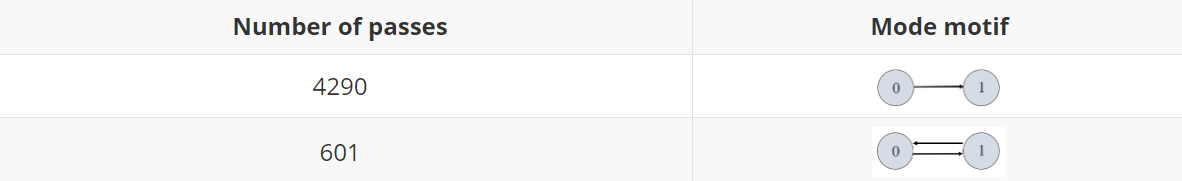
\includegraphics[width=0.75\textwidth]{figures/motif2.png}
		\caption{Statistics on the Occurrences of Different Mode Motifs of Dyadic Configuration}
		\label{fig:motif2}
	\end{figure}
	\begin{figure}[h]
		\centering
		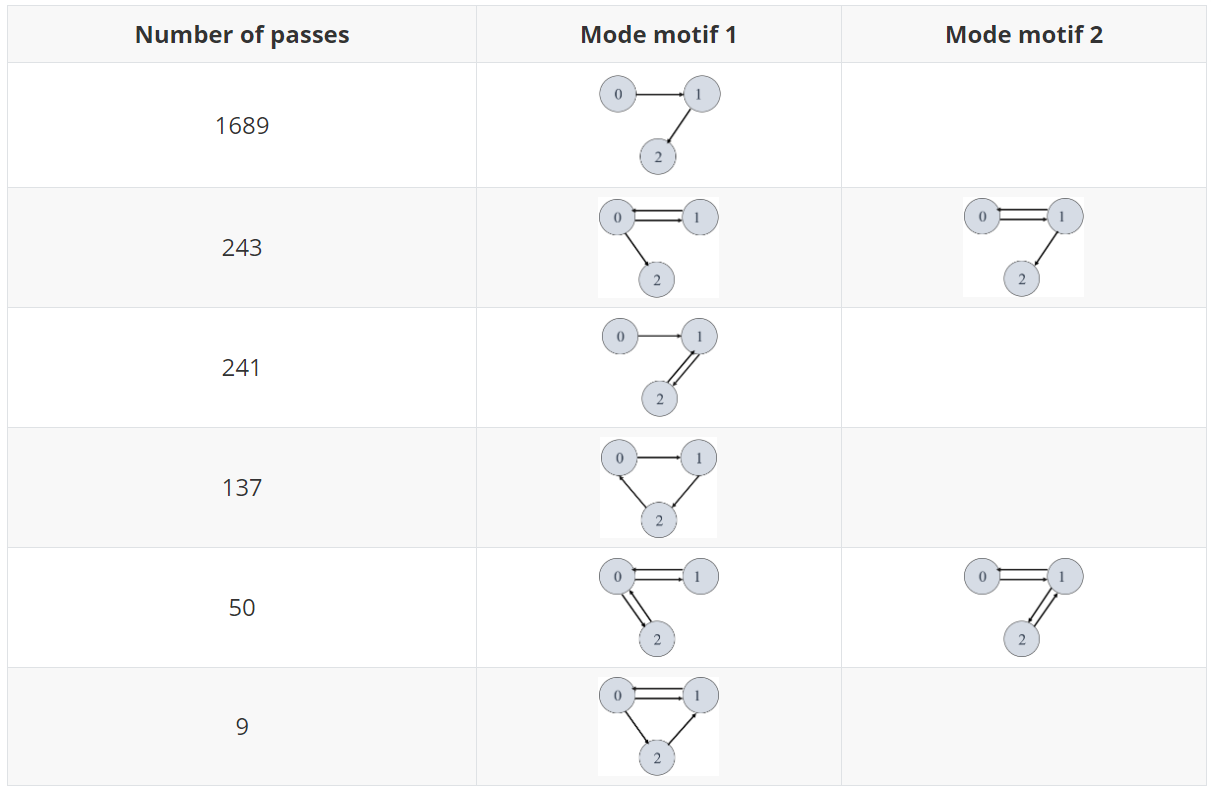
\includegraphics[width=0.75\textwidth]{figures/motif3.png}
		\caption{Statistics on the Occurrences of Different Mode Motifs of Triadic Configuration}
		\label{fig:motif3}
	\end{figure}
	
	We ignore the naive case that appears first in each configurations.  From figure \ref{fig:motif2} and figure \ref{fig:motif3}, we can intuitively see that in the case of dyadic configurations, the Huskies often use "0 - 1 - 0" and "0 - 1 - 0 - 1" mode motifs for passing.  For the triadic cases, it often uses "0 - 1 - 0 - 2", "0 - 1 - 2 - 1" and "0 - 1 - 2 - 0" mode motifs.  Compared with the longer dyadic and triadic chains, these passing mode motifs have more flexibility, but  can still be improved.

	In addition to dyadic and triadic configurations, we also select the case where the number of players is 4 as a representative of multiple configurations, and make statistics on the occurrence of its different mode motifs.  But because its number of mode motifs is far more than dyadic and triadic configurations, we put it in the appendices.
\subsubsection{Spatial Features}
	In this part, we have calculated the coordinates of the network centroid, the dispersion of the position of the players around the network centroid and advance speed of the Husky team's football passing network.  In order to make the results more general, we have calculated both the changes of these statistics per minute in a game, and the changes of these quantities in different games throughout the season.  Here are our statistics.

	We will analyze the statistics of a game first. Figure \ref{fig:game} shows the statistics of Huskies in a certain game.  From the coordinates of the network centroid, it can be seen that the Huskies players were closer to the opponent's goal in the second half, reflecting their fierce offensive in the second half.  It is clear by investigating the dispersion of the position of the players around the network centroid that the players are more concentrated in the second half, which confirms the opinion that the offensive in the second half is more fierce.  Judging from the advance speed, as the game progresses, the movement of the Huskies players is more inclined to go straight to the goal instead of a roundabout movement, which also confirms the previous opinion.
	\begin{figure}[h]
		\centering
		\begin{subfigure}[b]{0.24\textwidth}
			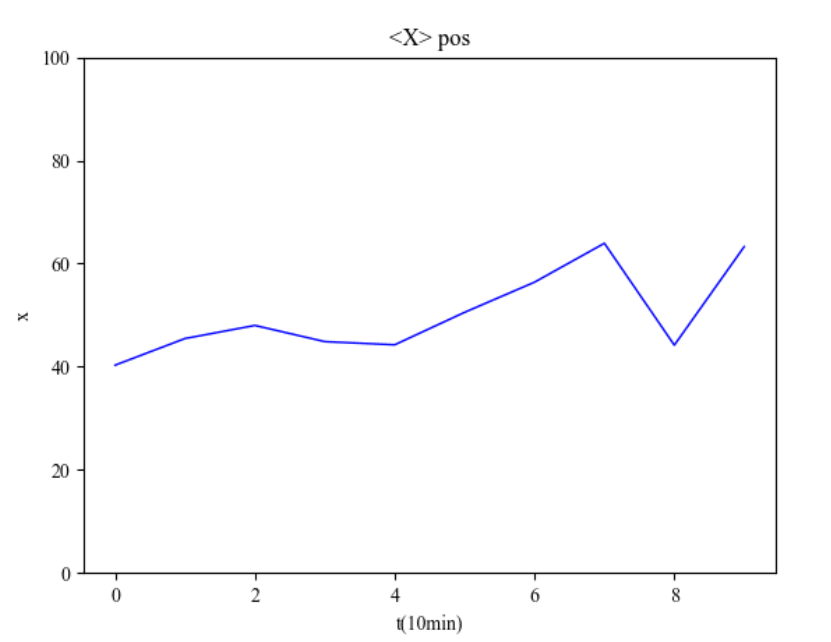
\includegraphics[width=\textwidth]{figures/xc1.png}
			\caption{X-coordinate.}
			\label{fig:x1}
		\end{subfigure}
		\begin{subfigure}[b]{0.24\textwidth}
			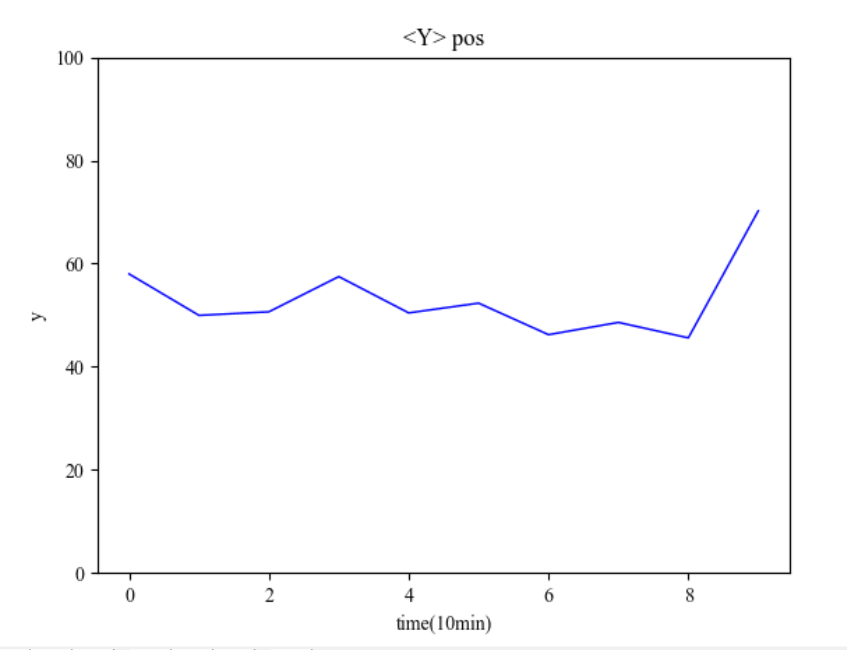
\includegraphics[width=\textwidth]{figures/yc1.png}
			\caption{Y-coordinate.}
			\label{fig:y1}
		\end{subfigure}
		\begin{subfigure}[b]{0.24\textwidth}
			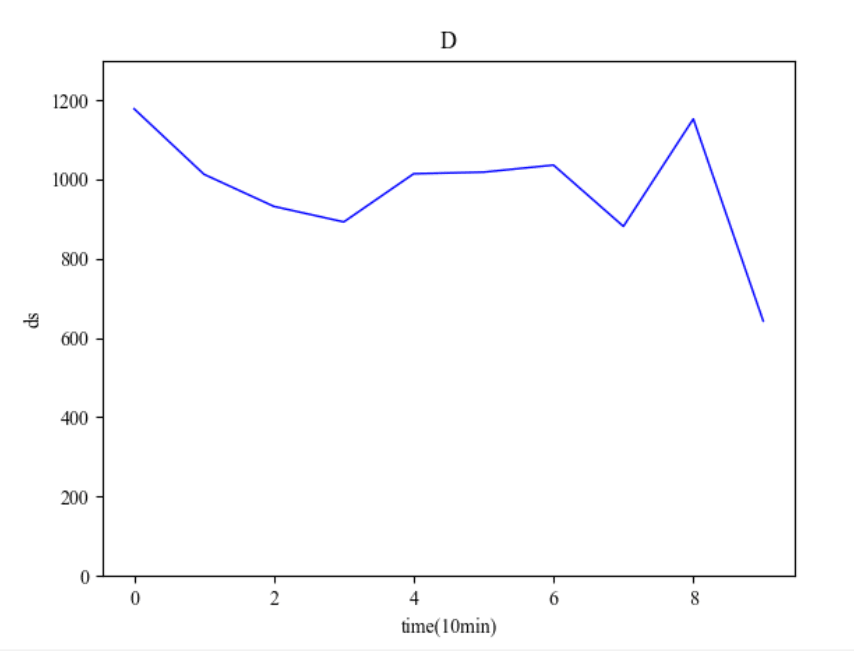
\includegraphics[width=\textwidth]{figures/d1.png}
			\caption{The Dispersion.}
			\label{fig:d1}
		\end{subfigure}
		\begin{subfigure}[b]{0.24\textwidth}
			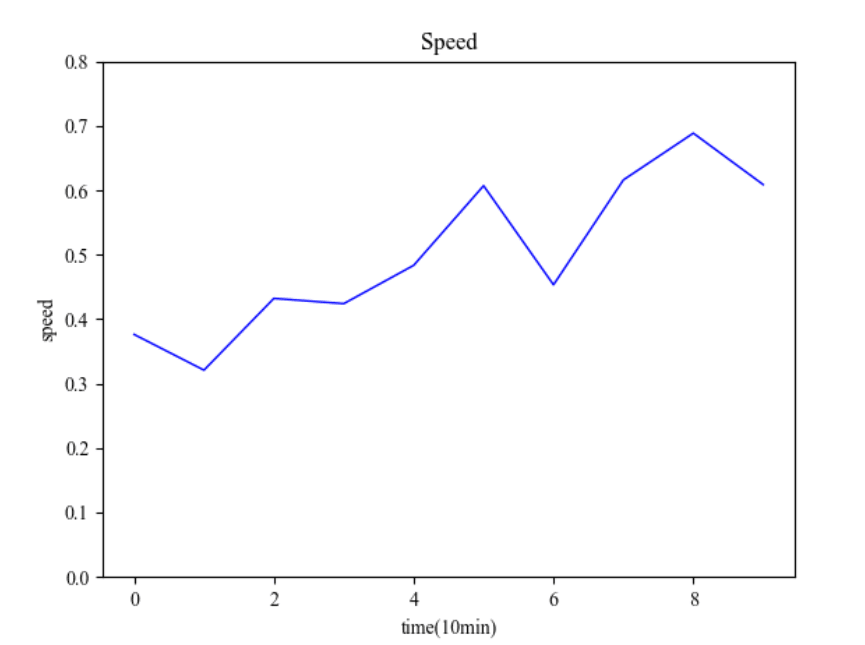
\includegraphics[width=\textwidth]{figures/s1.png}
			\caption{Advance Speed.}
			\label{fig:s1}
		\end{subfigure}
		\caption{The Change of Network Centroid's Coordinates, the Dispersion of the Position of the Players around the Network Centroid And the Advance Speed over Time in a Game.}\label{fig:game}
	\end{figure}

	After that, we can also analyze the changes in the spatial features of the Huskies players throughout the entire season.  It can be seen from Figure \ref{fig:season} that the coordinates of the network centroid are fluctuating throughout the season, but the amplitude of the fluctuations is not very large. It can be considered that the average spatial position of the Huskies players is relatively stable in all games throughout the season.  The change of thedispersion of the position of the players around the network centroid and advance speed throughout the season is more obvious, indicating that the spatial distribution density of the Huskies players and the direction of passes will make relatively clear changes with different opponents.

	\begin{figure}[h]
		\centering
		\begin{subfigure}[b]{0.24\textwidth}
			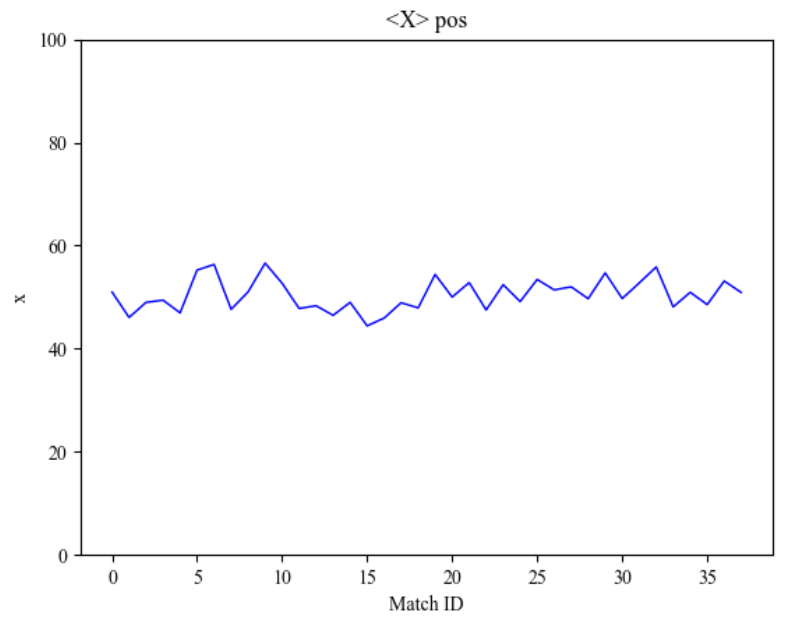
\includegraphics[width=\textwidth]{figures/xc2.png}
			\caption{X-coordinate.}
			\label{fig:x2}
		\end{subfigure}
		\begin{subfigure}[b]{0.24\textwidth}
			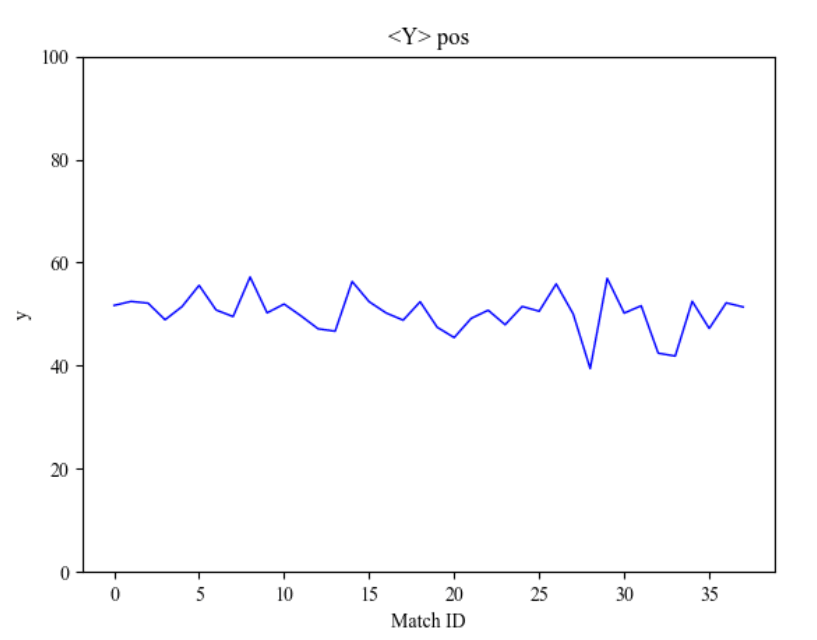
\includegraphics[width=\textwidth]{figures/yc2.png}
			\caption{Y-coordinate.}
			\label{fig:y2}
		\end{subfigure}
		\begin{subfigure}[b]{0.24\textwidth}
			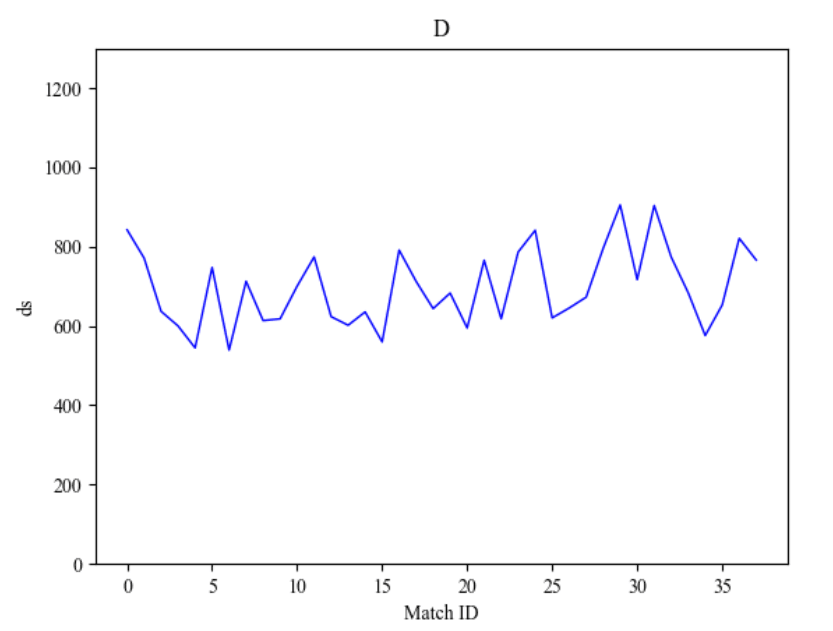
\includegraphics[width=\textwidth]{figures/d2.png}
			\caption{The Dispersion.}
			\label{fig:d2}
		\end{subfigure}
		\begin{subfigure}[b]{0.24\textwidth}
			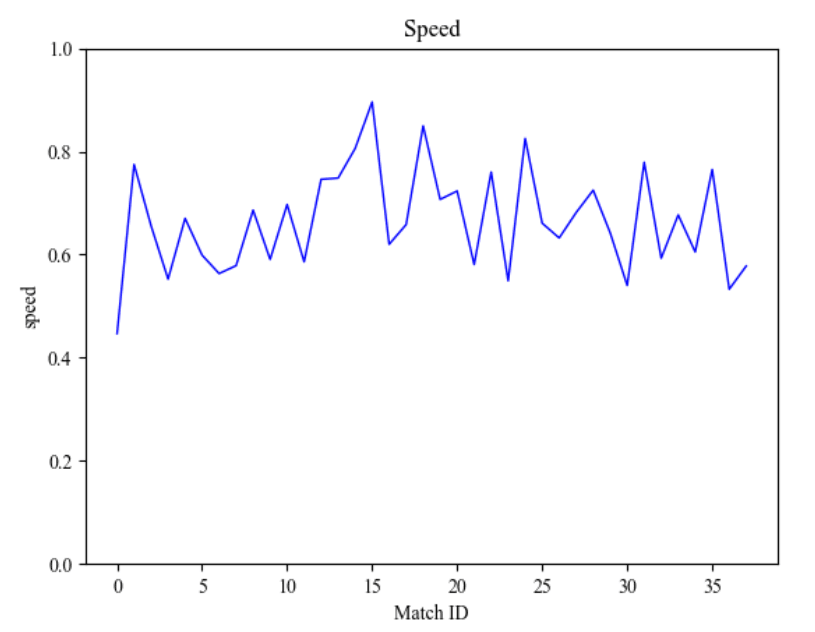
\includegraphics[width=\textwidth]{figures/s2.png}
			\caption{Advance Speed.}
			\label{fig:s2}
		\end{subfigure}
		\caption{The Change of Network Centroid's Coordinates, the Dispersion of the Position of the Players around the Network Centroid And the Advance Speed over Games in the Entire Season.}\label{fig:season}
	\end{figure}
\subsection{Teamwork Indicators}
\subsubsection{Calculation of indicators}
In the teamwork indicators model, we have 15 individual indicators in total. Most of them can be simply calculated according to the equations in section 4.3. For the shortest path matrix, we used the \textbf{Floyd Algorithm} to calculate the shortest path between every single point in the adjacency matrix.\par
After the calculation of the individual indicators, we summed them using the judgment matrix. First, we calculate the $CR=CI/RI$, which represents the consistency of the matrices, and found that they all meet the requirement: $CR<0.1$. Then, instead of calculating the weight vector using matrix eigenvalue extraction, we used a simplified algorithm to calculate its approximate weight matrix. First, normalize the column vectors of the judgment matrix separately. Then add the column vectors together to get a column vector. Finally, normalize this column vector and get the weight vector $\boldsymbol{\omega}$. After that, the row vector corresponding to each indicator $\boldsymbol{I_i}$ is arranged vertically to form an indicator matrix and we can calculate its weighted sum $\boldsymbol{I'}$ according to the equation:
$$
\boldsymbol{I}'=\boldsymbol{\omega}^T\left[\begin{matrix}
		\boldsymbol{I_1} \\
		\boldsymbol{I_2} \\
		\cdots \\
		\boldsymbol{I_n}
\end{matrix}\right]
$$
\subsubsection{Tactical analysis}
After the calculation of indicators, we can get detailed technical scores for each team. These indicators are of great significance in further tactical analysis. First, we listed these data (see appendix). Then we calculated the average value of each column and got some approximate results.\par

\begin{table}[htbp]
	\centering
	\label{table:teamwork_indicator}
	\caption{The average value of some of the items. (H represents Huskies and O represent the opponents)}
	\begin{tabular}{ccccccc}
	\toprule
	Item & Offensive-H &Offensive-O&Robustness-H&Robustness-O&Total-H&Total-O\\
	\midrule
	Average &-0.0428&0.0433&-0.3516&0.3516&-0.1315&0.1316\\ 
	\bottomrule
	\end{tabular}
\end{table}
\begin{figure}[htbp]
	\centering
	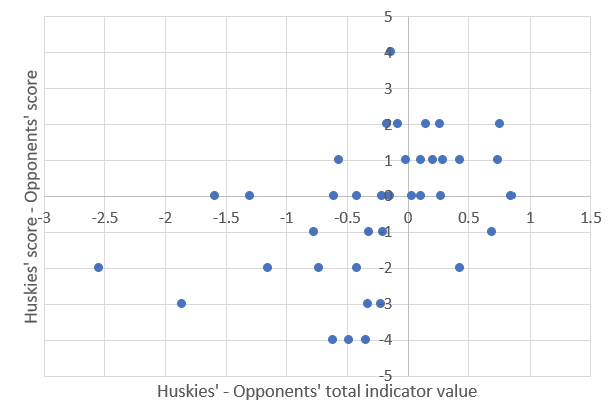
\includegraphics[width=0.4\textwidth]{figures/indicator_value.png}
	\caption{The relation between the team's score and the indicator value.}
	\label{fig:indicator_value}
\end{figure}

We find that most of the points in (Fig. \ref{fig:indicator_value}) are in the first and third quadrants, which shows that \textbf{the model of the evaluation index is valid from one game to the entire season}. Thus we can use these indicators to evaluate the performance of the players in each game and give better strategies.\par


\begin{figure}[h]
	\centering
	\begin{subfigure}[b]{0.16\textwidth}
		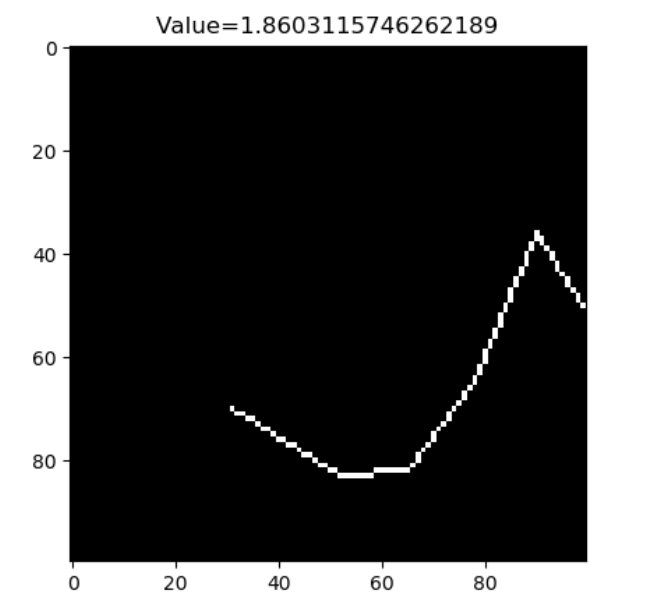
\includegraphics[width=\textwidth]{figures/shot1.png}
		\caption{1st.}
	\end{subfigure}
	\begin{subfigure}[b]{0.16\textwidth}
		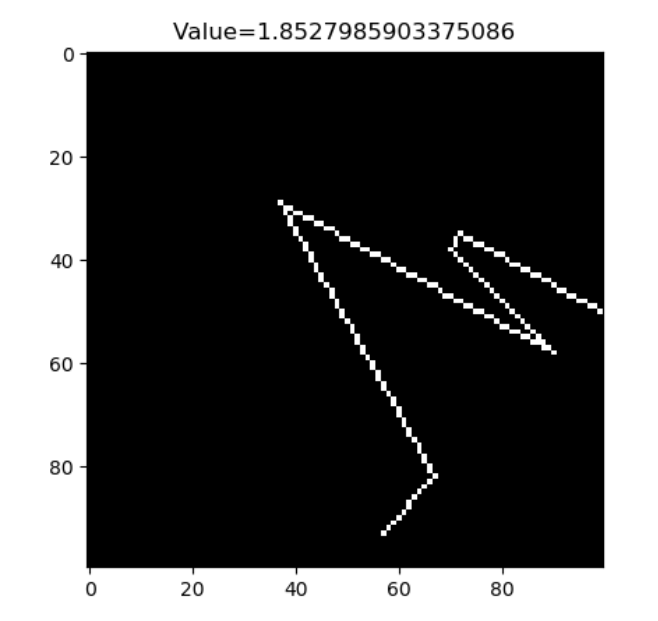
\includegraphics[width=\textwidth]{figures/shot2.png}
		\caption{2nd.}
	\end{subfigure}
	\begin{subfigure}[b]{0.16\textwidth}
		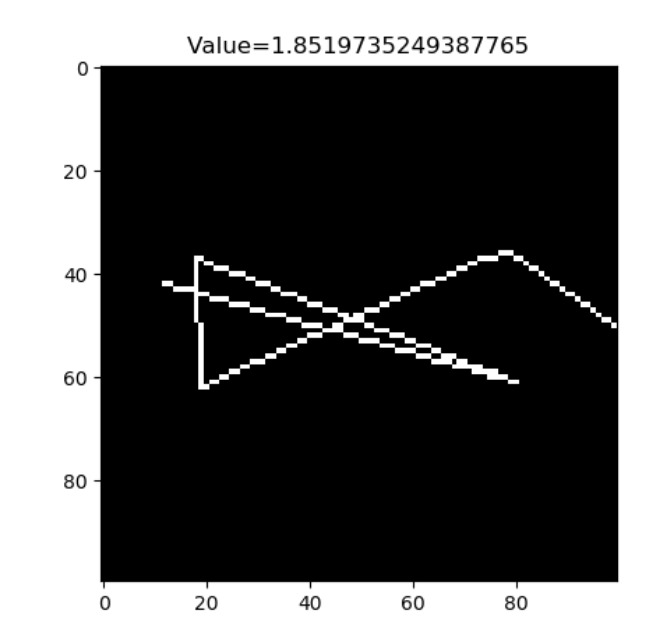
\includegraphics[width=\textwidth]{figures/shot3.png}
		\caption{3rd.}
	\end{subfigure}
	\begin{subfigure}[b]{0.16\textwidth}
		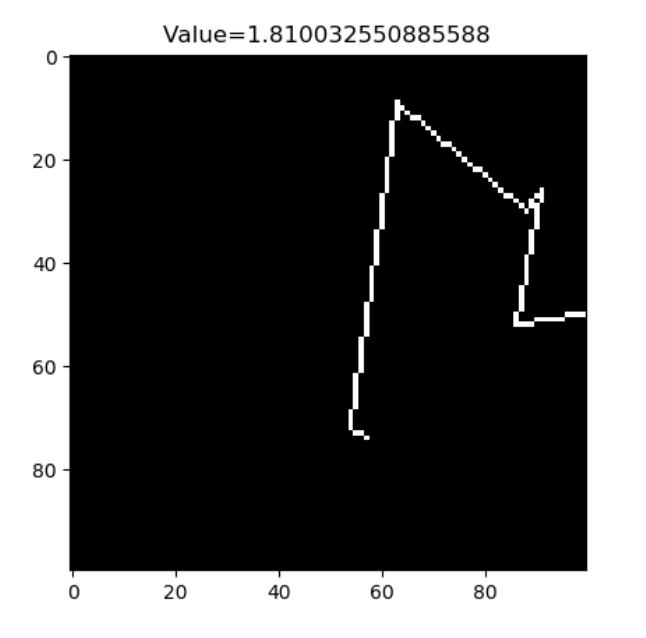
\includegraphics[width=\textwidth]{figures/shot4.png}
		\caption{4th.}
	\end{subfigure}
	\begin{subfigure}[b]{0.16\textwidth}
		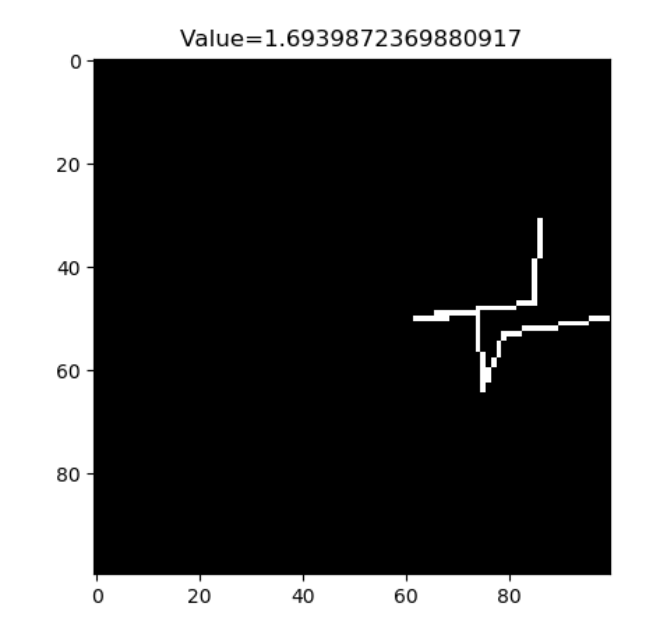
\includegraphics[width=\textwidth]{figures/shot5.png}
		\caption{5th.}
	\end{subfigure}
	\begin{subfigure}[b]{0.16\textwidth}
		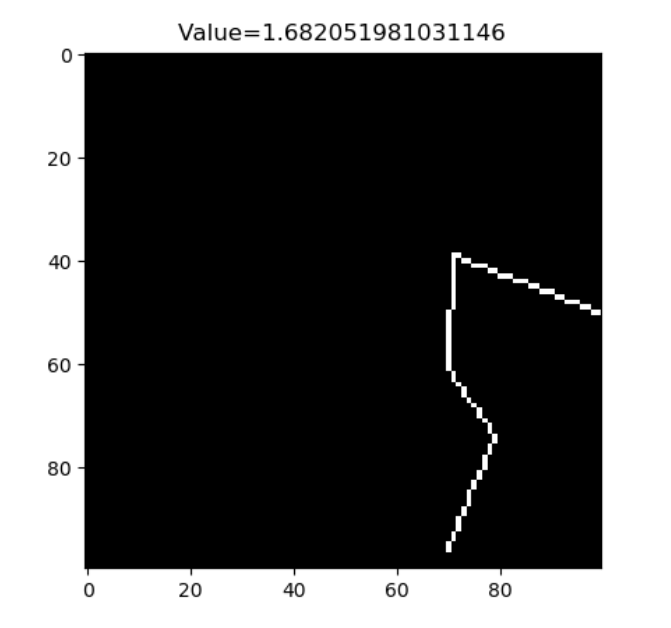
\includegraphics[width=\textwidth]{figures/shot6.png}
		\caption{6th.}
	\end{subfigure}
	\caption{Some of the highest rated goals.}
	\label{fig:highest_goal}
\end{figure}

We recorded the highest rated offensive routes (Fig. \ref{fig:highest_goal}) to analyze their offensive strategies. We tried to use the deep neural network to extract its features in order to summarize the offensive skills, such as the GAN, AutoEncoder and CNN. In GAN and AE network, the images generated by the neural network showed the features that were too single, which made it relatively difficult to study their characteristics. So we finally gave up using neural network methods to extract features and used the method of induction and summary to conduct a detailed analysis of high-scoring offensive routes, which are introduced in section 6 in detail.


\section{Structural Strategies}
\subsection{Offensive tactics}
\begin{enumerate}[(1)]
	\item \textbf{Backcourt}.\par
	\qquad Outstanding team offenses are looking for opportunities and seizing opportunities to attack. Therefore, the strong team's ball possession rate is generally maintained at a high level. And the strong team's passing network can be seen, their defenders pass the most. A good player should seize the opportunities rather than afraid of waste of time. By passing each other back, grasping the ball can not only relieve the pressure, but also create good offensive opportunities. \par
	\qquad The back pass is often used in football games. It can not only play a tactical role in local cooperation, but also give strategic significance to the situation in the entire court. Offensively, by passing back the ball, you can flexibly grasp the offensive direction, adjust the rhythm of the game, and mobilize the opponent. Take advantage of the loopholes in the opponent's transfer to seek shooting opportunities and create conditions for scoring. Therefore, it is necessary to increase the proportion of guards transmitting the ball to each other and exercise precision and non-stealth.
	\begin{figure}[h]
		\centering
		\begin{subfigure}[b]{0.45\textwidth}
			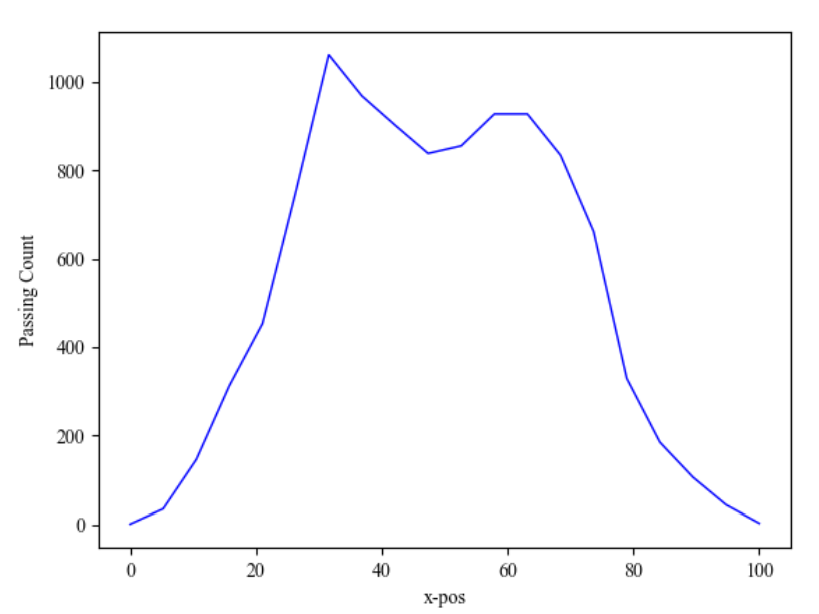
\includegraphics[width=\textwidth]{figures/backcourt.png}
			\caption{The team's number of passes changes with the x coordinate.}
			\label{fig:backcourt}
		\end{subfigure}
		\begin{subfigure}[b]{0.45\textwidth}
			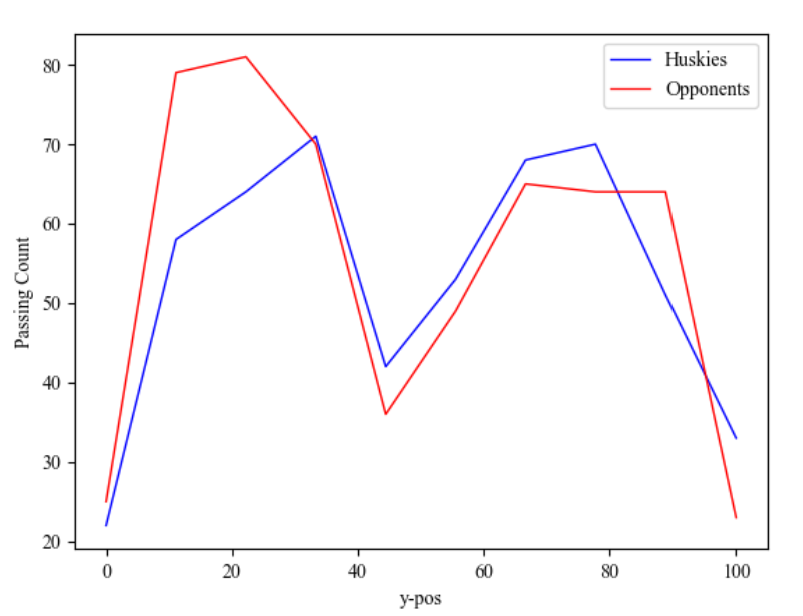
\includegraphics[width=\textwidth]{figures/backtofront_pos.png}
			\caption{The passing count of the passing in the middle and on the side. }
			\label{fig:back_to_front}
		\end{subfigure}
		\label{fig:passing_count}
		\caption{The passing count position.}
	\end{figure}
	\item \textbf{Continuous pass.}\par
	\qquad It can be seen from the data that triangle tactics are used the most and can also achieve good results. Continuous passes can allow opponents to run out of gear before they react, and they can excel without confrontation. Good passing coordination can even bypass the opponent's defensive line and enter the dangerous position for shooting. In the midfield, you can also use a straight pass to cooperate with the two-on-one. Therefore, it is necessary to increase the ability of forwards and wing centers to respond, and continuously forward the ball to make it easier for the forward to pass through the defense line of the opposing defender.
	\item \textbf{Sidewalk alternation.}\par
	\qquad Don't focus too much on the middle. Although the area of the middle is large and the angle is good, it is also the main force of the opponent's defense. So more opportunities are created in the sidewalks, and active crossovers can play an unexpected role. By analyzing the lost games of the Huskies, it can be seen that most of the opponents are active wing alternates to make it easy to dissolve the Husky's back line of defense. Therefore, for the purpose of learning from others, the front lines on the left and right should actively run without the ball to create opportunities for passing in the middle and communicate with each other. This can largely tear the defense of the team with poor defense line.
	\item \textbf{Short and long passes work together}\par
	\qquad After a large number of short passes, the sudden high ball often caught the opponent by surprise. The offensive player only needs to occupy the place in advance to easily tear the opponent's defensive line to bring the ball into the penalty area. The strong team's ball network can often see a large range of ball, which not only can make a sudden change in rhythm so that the opponent can not cope, and can easily send the ball to the opponent's penalty area.\par
	\qquad In addition, there is the forward's response and ability to grab positions. Being able to run to the ball in time is an important ability requirement for the forward. In addition to the large-scale Cross, another popular high kick in football today is long corner kicks. At this stage, long-distance corner kicks have become a key part of strong team tactics. If it is difficult to enter the penalty area, you can choose to win the corner by creating an opponent player out of bounds. Find opportunities to score in the long corner. At that time, the centers will all come up to help the forwards. This will be much easier than the striker's cooperation into the restricted area. Therefore, you should train long-distance conductive balls to increase the large-scale conductive balls in the network.
	\begin{figure}[htbp]
		\centering
		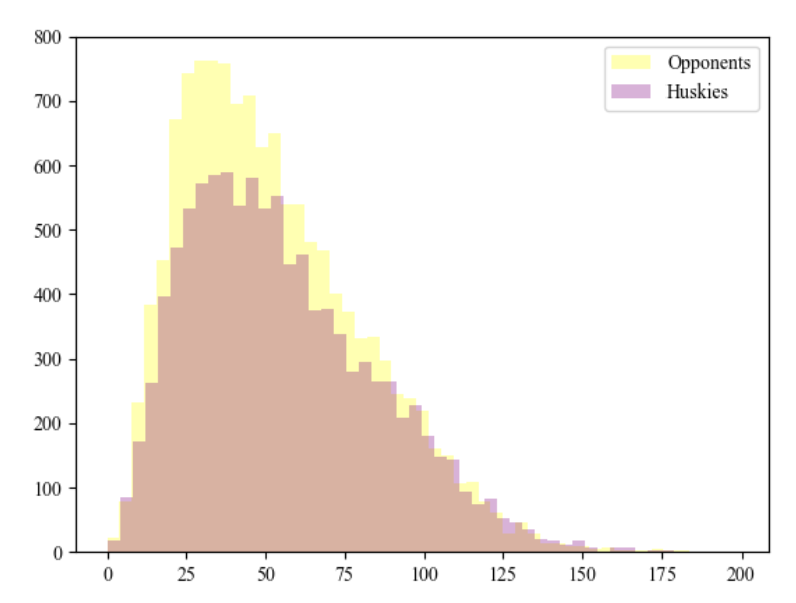
\includegraphics[width=0.5\textwidth]{figures/passing_cnt.png}
		\caption{The passing distance count for Huskies and the opponents. The opponents have more passings than Huskies and the average distance of passing is a bit smaller than  the Huskies.}
		\label{fig:passing_cnt}
	\end{figure}
	\item \textbf{Reduced Short Corners}\par
	\qquad Near the corner, the player quickly passed the ball to the forward teammate, and cooperated with the back pass to complete the shot. Short-kick corner kicks extend the time of the offense because they must be launched after the coordinated pass. While the same team members select positions, the opposing defensive players and goalkeepers' positions will be more accurate, thereby forming a good defensive formation. This is not conducive to grab a point attack. Therefore, in many cases, short corner kicks are issued quickly when the opponent's defensive position is not tight to gain a short-term advantage in time and space, and seek better passing points through passing. But at this stage, the strong teams' defense lines are very solid, so it is difficult to find such opportunities. Therefore the number of short corner kicks should be reduced.
\end{enumerate}
\subsection{Defensive Strategy}
\begin{enumerate}[(1)]
	\item \textbf{Pressure defense.}\par
	\qquad The teams that conceded less goals reacted particularly quickly when they turned defense. Once the team loses the ball in the midfield and frontcourt, it immediately organizes the defense. The loser quickly blocks the interceptor, and the other defensive players apply close marks to the attacking players who come to respond. This is called pressure defense. The oppressive defense emphasizes the immediate use of snatching and organization of defense at the moment of transition from offense to defense, making up for the loopholes generated when the defense is weak at the moment of offense and defense transition, and limiting the opponent's counterattack. This requires the striker to develop the ability to steal and the center to follow the forward quickly to make the enemy's passing network constrained in the enemy's half-court area.
	\item \textbf{Zone defense and tight defense.}\par
	\qquad In the game, there are more mixed defenses combining zone defense and pressing man-to-man. The advantage of man-to-man defense is that it is hard to attack the offensive players. However, the defensive gap is often caused by the offensive players' conscious crossover and response. Combining with zone defense can make up for this shortcoming. When the offensive player crosses the position, the defensive player can exchange views without changing the position. When the ball is still far from the goal, each person is responsible for an area and the opponent player have no chance to run. Once the opponent starts to attack, we should pull the defensive line back and choose the strategy of pressing on people, forcing the opponent's offensive line to break through our defensive line. The two most common types of man-to-man tactics are the three-backer's two strikers against each other and the use of man-to-man defensive tactics in corner defense.
\end{enumerate}
\subsection{Formation}
\begin{figure}[h]
	\centering
	\begin{subfigure}[b]{0.24\textwidth}
		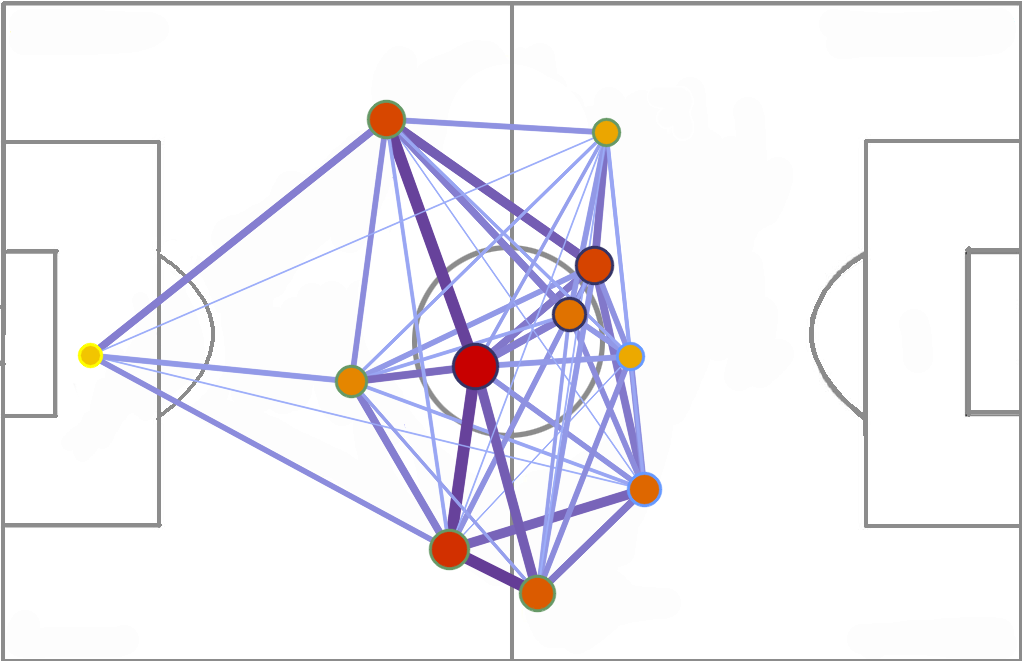
\includegraphics[width=\textwidth]{figures/win_team1.png}
		\caption{Match 9.}
		\label{fig:win_team1}
	\end{subfigure}
	\begin{subfigure}[b]{0.24\textwidth}
		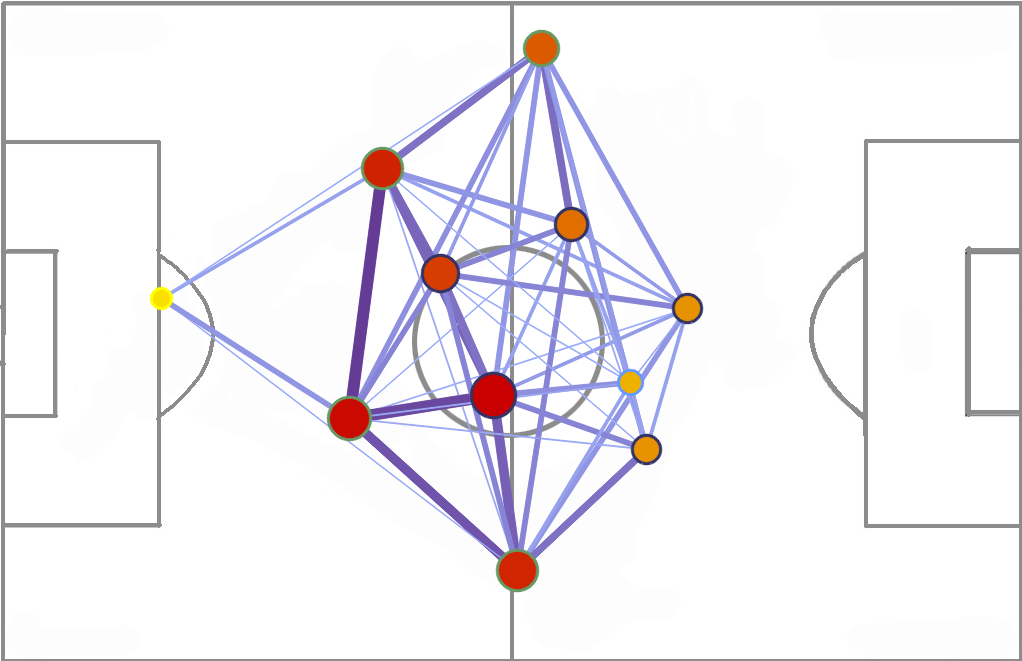
\includegraphics[width=\textwidth]{figures/win_team2.png}
		\caption{Match 13.}
		\label{fig:win_team2}
	\end{subfigure}
	\begin{subfigure}[b]{0.24\textwidth}
		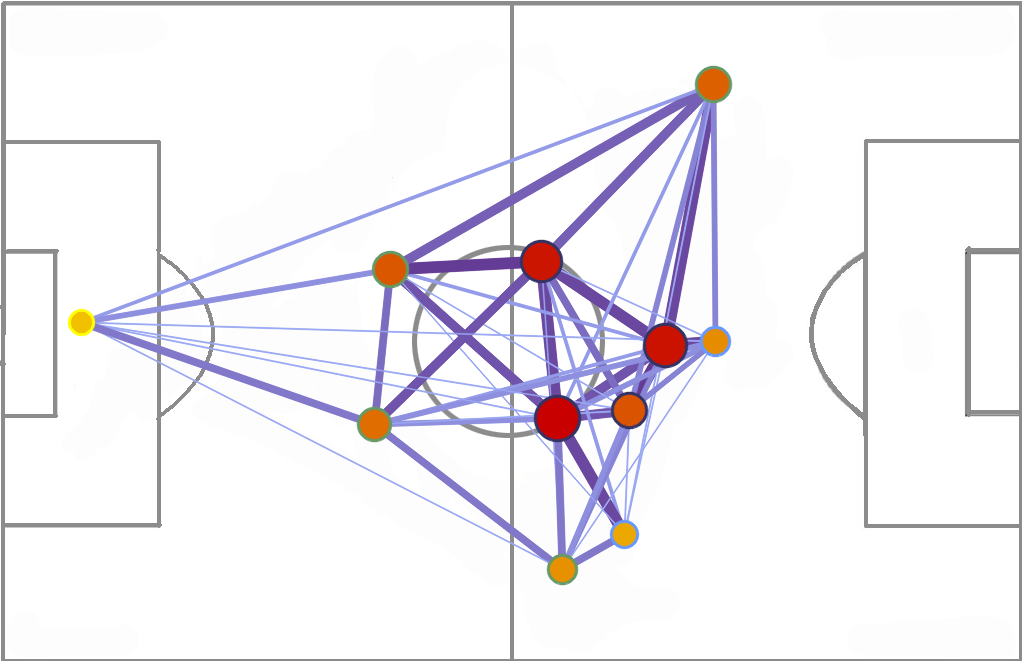
\includegraphics[width=\textwidth]{figures/win_team3.png}
		\caption{Match 23.}
		\label{fig:win_team3}
	\end{subfigure}
	\begin{subfigure}[b]{0.24\textwidth}
		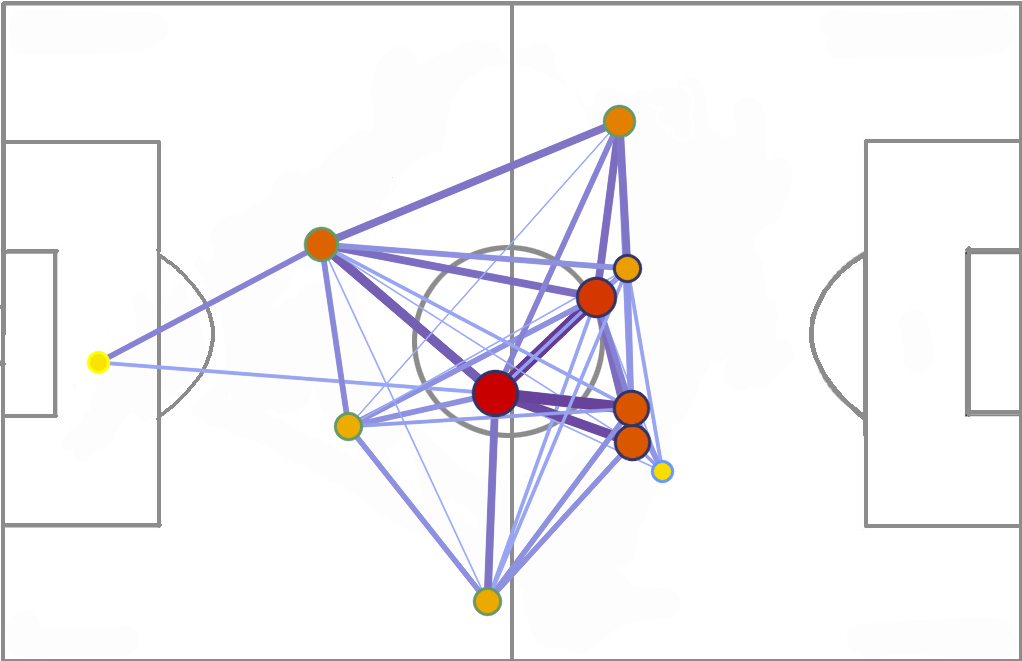
\includegraphics[width=\textwidth]{figures/win_team4.png}
		\caption{Match 26.}
		\label{fig:win_team4}
	\end{subfigure}
	\caption{Formation of the teams that gained a great advantage in the game against the Huskies.}
	\label{fig:win_team}
\end{figure}
We analyzed the formation of the teams that gained a great advantage in the game against the Huskies (Fig.\ref{fig:win_team}). According to our model in section 4.3, we calculated the score of each item in these four games. The result showed that the four winning teams scored 0.15, -0.01, and 1.33 points on offense, defense, and robustness, which far exceeded the Husky's -0.12, -0.66, and -0.67 points. We found some significant features in those formations of the teams.\par
\textbf{Parallel positions.} The formations are mainly parallel positions, and the offense and defense are extremely balanced. In these formations, it is easy to dispatch and the attack is easy to sort out.\par
\textbf{More midfield players.} There are more people in the midfield to ensure smooth running and transfer of the ball. When the attack was overwhelming, a pressure-type attack was performed in the opponent's half. At the same time, because of the large number of midfielders, they can better kick out and make changes according to the situation. And the two wingers are extremely flexible, and their moves will not damage the defensive structure of the middle.\par
\textbf{More triangle offenses.} Throughout the formation, there is a close connection between the back and front waist. The success rate of triangular pass penetration is more effective than the straight pass, and it is also flexible. So the frontcourt player can retreat or return to his own half at any time. Furthermore, a sufficient number of potential offensive players means that the entire formation will not lose pressure on a defensive counterattack when a player is behind.
\par
In general, the formation of these teams helps the team to attack quickly and effectively prevent the opponents from counterattack in the middle. And it helps the team to be more robust.

\subsection{Method to Design More Effective Teams}
	Based on the concept of "job crafting", we propose the concept of "team crafting" for teamwork.  "Team crafting" means that team members work together to decide what or how to change their work through close collaboration and communication.  It is noted that "team crafting" research is quite necessary:
	\begin{itemize}
		\item At present, the remodeling of team work is a common phenomenon in organizations. In modern organizations, teams have gradually become the basic unit of work.  Organizations complete complex work tasks through teams, increasing organizational flexibility and improving overall performance.
		\item Reshaping teamwork will be better for organizational needs.  There is a certain difference between individual work remodeling and team work remodeling. The remodeling of individual work is led by individual employees. The purpose is to achieve better personal-job matching.  But if personal goals and organizational goals are inconsistent, employee job remodeling may have a negative impact on the collective. However, the main body of team remodeling is the team members as a whole, which can better realize the overall interests of the team.  Therefore, the remodeling of teamwork will achieve a better balance between organizational interests and individual interests.
	\end{itemize}

	The mechanism of the model given below is based on the analysis of the first two questions, and will finally tell us how to design a more effective team.

	\begin{enumerate}
		\item Conceptual connotation and measurement
		
		\qquad The focus adjustment represents the way in which individuals take action in the face of the goals and outcomes they are pursuing, and may affect people's preferences and choices in life.  The adjustment focus can be divided into two different motivation systems, namely promotion focus and prevention focus.  The former means that individuals pay more attention to cultivation, growth and achievement, while the latter means that individuals pay more attention to protection, safety and responsibility.

		\qquad Based on the theory of regulating focus, team crafting is divided into facilitation team work remodeling and defensive team work remodeling.  Note that this variable is two independent variables, not the two ends of a variable, so there will be double high, double bottom and one high and one low.

		\item Antecedent mechanism
		
		\qquad According to the IMOI (Input-Mediator-Outcome-Input) team operation model, the input variables at the individual, team, and organization levels pass through the team mediation process to generate team outputs.  Therefore, the antecedent variables include leadership behavior, team personality composition, team work characteristics, and cooperative human resource management system.

		\begin{itemize}
		\item Leadership behavior
		
		\qquad Leadership behavior is divided into transformational leadership and transactional leadership.  The transformational leader's role as a change agent will encourage the team to continue to try, pursue growth and progress, and show more motivating team work to reshape behavior.  Transactional leaders emphasize the completion of job responsibilities and compliance with norms, encourage the team to pursue stability and security, and the team shows more defensive team work to reshape behavior.

		\item Team personality
		
		\qquad The adjustment focus and initiative personality of team members will affect the remodeling of team work.  The average promotion focus of team members is positively related to the remodeling of facilitative team work, and the average defense focus of team members is positively related to the remodeling of defensive team work.  In terms of proactive personality, the mean value of team proactive personality is positively related to the remodeling of facilitative teamwork and negatively related to the remodeling of defensive teamwork.

		\item Team work characteristics
		
		\qquad Team work autonomy and team task interdependence have a positive impact on both types of team work remodeling.

		\item Cooperative Human Resource Management System
		
		\qquad Organizational cooperative human resource management system will positively affect team remodeling.
		\end{itemize}

		\item Initiative Research Perspective
		
		\qquad The team's active motivation states include three states: can do, reason to, and energized to.  Corresponding to the team's collective effectiveness, team identity, team positive emotional atmosphere.

		\item Dynamic perspective
		
		\qquad Team work commitment and team cohesion play an intermediary role between team remodeling and team effectiveness.  Over time, after team work remodeling affects team work input and team cohesion, these team states and processes will in turn affect team work remodeling, and then propose a two-way interaction of team work remodeling and team work input and team cohesion  Mechanisms.

	\end{enumerate}

	Therefore, we propose the following idea:
	\begin{figure}[h]
		\centering
		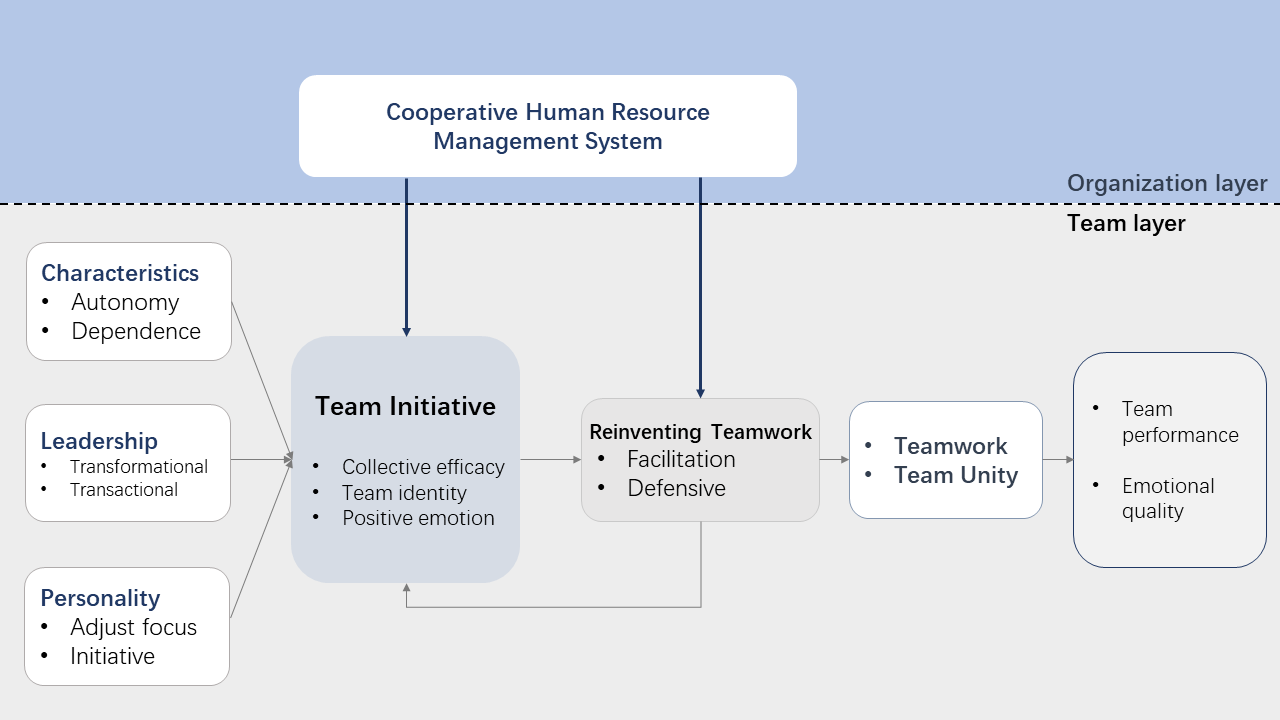
\includegraphics[width=0.75\textwidth]{figures/HR.png}
		\caption{The Schematic Diagram of the Team Crafting Model} 
		\label{fig:teammodel}
	\end{figure}

	Hence an effevtive team should consider these points:
	\begin{itemize}
	\item The problem-solving process should have some autonomy, and the problem can be split into sub-problems and their dependencies should not be particularly tight.
	\item Leaders need to be transformative, that is, they will encourage the team to continue to try, pursue growth, and pursue progress.  Therefore, the team is more likely to set higher goals, seek more opportunities and challenges, expand the scope of tasks, and strive for more resources.
	\item The team should have both a personality that promotes focus and a personality that defends focus, and everyone should have a team initiative personality.
	\item Leaders should communicate more with team members to promote their collective identity and create a positive emotional atmosphere.
	\item At the same time, we should pay attention to each member's areas of expertise and learn from each other's strengths.
	\end{itemize}
	
\section{Model Analysis}
\subsection{Sensitivity Analysis}
In our model, the most sensitive part is the judgment matrix, which was totally generated by our experience. Although it is easy for us to judge the importance between to items, we are not able to clearly identify their exact values. Thus we are supposed to perform a sensitivity analysis to test the reliability of the model.\par

\begin{table}[htbp]
	\centering
	\label{table:sensitive}
	\caption{The average value of some of the items before and after changed. (H represents Huskies and O represent the opponents)}
	\begin{tabular}{ccccccc}
	\toprule
	Item & Offensive-H &Offensive-O&Robustness-H&Robustness-O&Total-H&Total-O\\
	\midrule
	Origin &-0.0428&0.0433&-0.3516&0.3516&-0.1315&0.1316\\ 
	Changed &-0.0448&0.0453&-0.3516&0.3516&-0.1206&0.1207\\ 
	\bottomrule
	\end{tabular}
\end{table}

In order to test the sensitivity of the judgment matrices, we changed some of the values in the matrices and ensure them meet the consistency requirements. Then we ran the model in section 4.3 again and compared them with the origin ones. We found that the difference between the two results is small, which means that the model has low sensitivity to the judgment matrix.

\subsection{Strengths and Weakness}
\section{Conclusion}

\bibliography{ref}
\newpage

\begin{appendices}

\section{Mode Motifs for Multiple Configurations}

\begin{figure}[h]
	\centering
	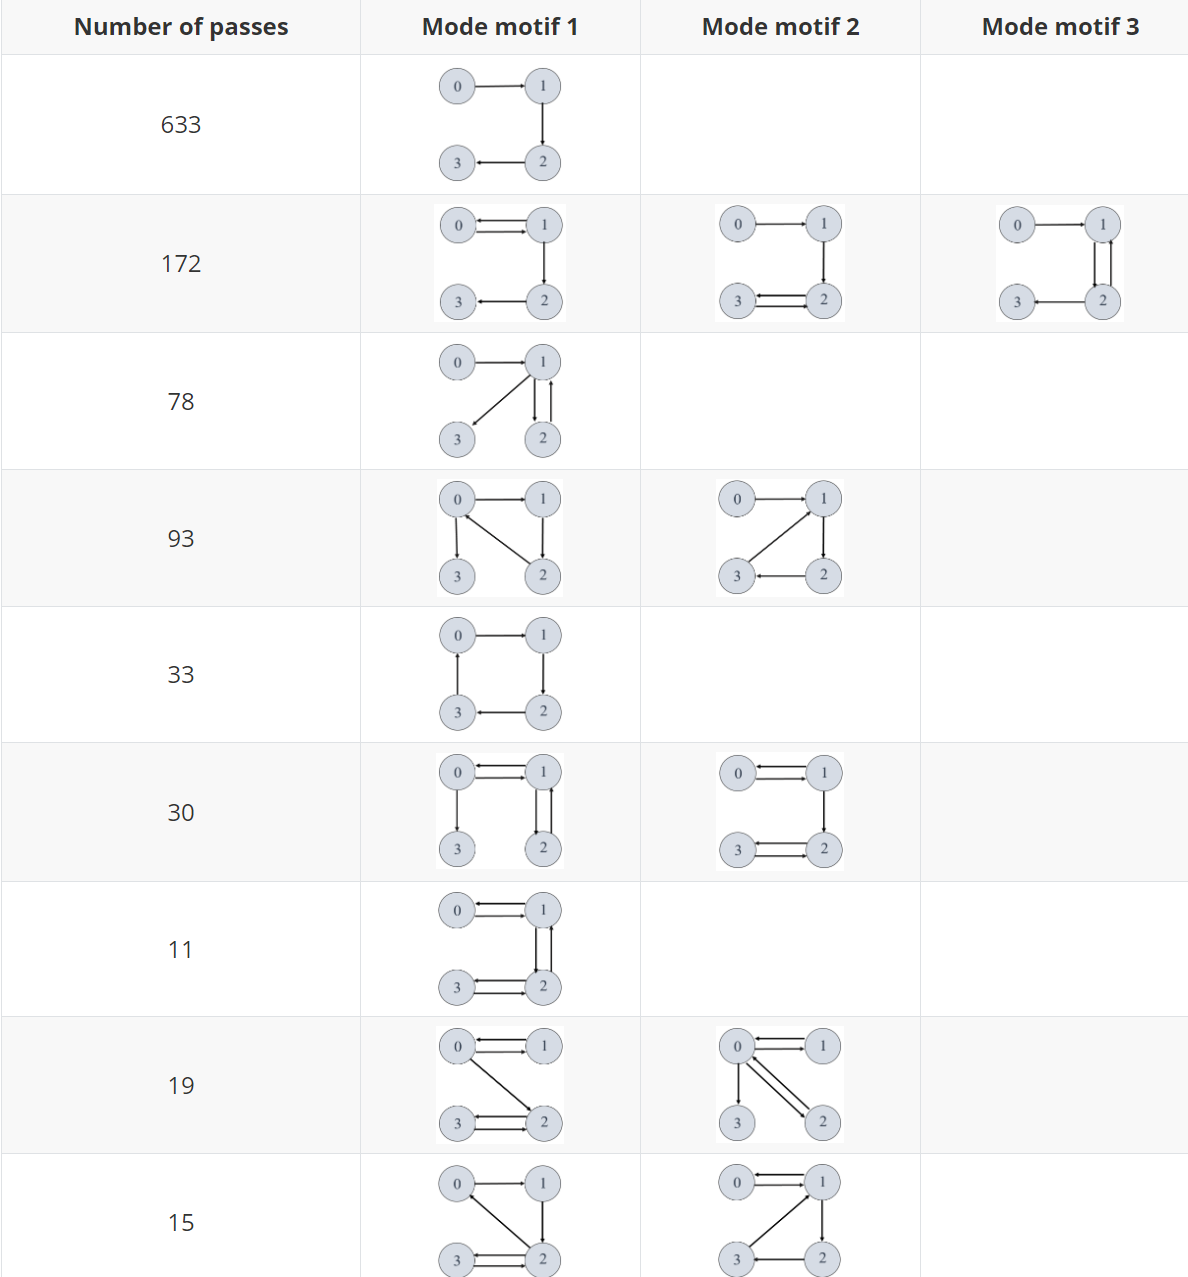
\includegraphics[width=\textwidth]{figures/motif4.png}
	\caption{Mode Motifs for Multiple Configurations}
	\label{fig:motif4}
\end{figure}

\section{Code}
\subsection{Problem One}
\inputpython{code/problem1_solve1.py}{1}{72}
\inputpython{code/problem1_visual1.py}{1}{123}
\inputpython{code/problem1_visual2.py}{1}{106}
\inputpython{code/problem1_high_chart.py}{1}{41}
\subsection{Problem Two}
\inputpython{code/problem2_gan.py}{1}{150}
\inputpython{code/problem2_solve1.py}{1}{361}
\inputpython{code/problem2_visual1.py}{1}{80}
\inputpython{code/AHP_utils.py}{1}{63}
\inputpython{code/problem_ae.py}{1}{88}
\subsection{Problem Three}
\inputpython{code/problem_visual3.py}{1}{104}
\end{appendices}

\end{document}
